\section{Results: Locating the Failure}
\label{sec:locating}

\subsection{The Failure Is Structural: Selective Substitution on Compound-Jump Commands}

The compound-jump test set contains 7706 examples. At the checkpoint used throughout
this work (S-043), T5-small achieves 43.2\% accuracy (3330/7706), for a failure rate
of 56.8\% (4376 failures). This is not random degradation: the encoder marks
\texttt{jump} as categorically distinct from trained primitives at layer 5
($p = 0.0000$, Mann--Whitney, experiment S-043), confirming that the failure occurs
despite encoder awareness of the OOD primitive, not because of encoder blindness.

S-047 shows that the failures are structurally concentrated.
Figure~\ref{fig:failure-rate} (\S\ref{sec:intro}) breaks down failure rate by structural
command feature: commands containing \texttt{around} fail at 87.3\%
(\texttt{has\_around}=1) versus 22.4\% for commands without it (lift $= +0.648$,
AUC $= 0.806$, $\chi^2$~$p = 0.0000$, $n = 200$).
The pre-registered hypothesis that \texttt{has\_after} (argument-order reversal) would
dominate was incorrect: \texttt{has\_after} contributes lift $= +0.083$, AUC $= 0.572$,
$p = 0.297$ --- not distinguishable from noise.
The actual dominant structure is the four-cycle identity morphism:
\texttt{jump around left} requires four turn-action cycles,
$({\tt I\_TURN\_LEFT}\ {\tt I\_JUMP}){\times}4$,
with the OOD primitive in the action slot of each cycle.

The dominant failure mode is \emph{substituted-walk}: T5 generates
$({\tt I\_TURN\_LEFT}\ {\tt I\_WALK}){\times}4$ --- correct cycle count, correct cycle
structure, wrong action token.
This represents 13 of 50 sampled \texttt{has\_around}=1 failures (26\%, S-049).
Critically, zero failures are of the \texttt{half\_count\_2of4} type (the ``180$^\circ$
hypothesis''): T5 does not miscount the cycles. It counts correctly and substitutes.
The failure target is therefore well-defined: explain why the action slot is filled with
\texttt{I\_WALK} instead of \texttt{I\_JUMP}, given that the cycle structure is correct.

\subsection{Routing Is Not the Primary Discriminator in the Stored Comparison (S-049)}

Having established that the failure is structural and occurs in the decoder, the first
mechanistic question is whether the decoder is routing its cross-attention correctly ---
that is, whether it attends to the relevant encoder position when selecting the action token.

S-049 captured decoder cross-attention weights during generation for two groups:
\texttt{has\_around}=1 fail ($n = 50$) and \texttt{has\_around}=1 success ($n = 25$).
The hypothesis that failing cases would show lower attention to the \texttt{around}
encoder position is not supported.

\begin{quote}
Fail group: mean cross-attention to \texttt{around} $= 0.106$.
Success group: mean cross-attention to \texttt{around} $= 0.103$.
Mann--Whitney $p = 0.9208$ (not significant).
\end{quote}

The stored routing summary did not discriminate fail from success in this comparison.
Figure~\ref{fig:routing-summary} shows this comparison across all six decoder layers
and in aggregate (h1): the per-layer attention weight profiles for fail and success are
nearly identical, with peak divergence at layer 4 (stored in sealed JSON as
\texttt{max\_divergence\_layer = 4}) and no consistent directional difference.
The same comparison framework did detect a significant secondary difference elsewhere:
fail cases show \emph{higher} cross-attention entropy relative to the control group
(A $= 1.434$ vs. C $= 1.357$, $p = 0.0017$, S-049 H3).
Failing cases distribute attention more diffusely across encoder positions, but this
does not explain the specific substitution to \texttt{I\_WALK}.
Because the framework can register a difference when one is present, the null routing
result is treated as evidence that routing is not the primary discriminator in this
comparison, not as a blanket proof of equivalence.

Routing is not the primary discriminator in this stored comparison.
The failure occurs downstream of cross-attention routing.

\begin{figure}[t]
\centering
\includegraphics[width=\linewidth]{figures/fig02_decoder_routing_summary}
\caption{Decoder routing summary by layer, T5-small SCAN \texttt{add\_prim\_jump}
(S-049). Summary statistics only; full attention matrices not available.
Panel~(A): Mean cross-attention weight per decoder layer (L0--L5) for fail ($n=50$)
and success ($n=25$) groups; profiles nearly identical across all layers.
Peak divergence at L4 (stored in sealed JSON).
Panel~(B): h1 aggregate comparison; mean attention to \texttt{around} token is
statistically indistinguishable ($p=0.9208$, NS).
K1: routing profiles similar in fail and success cases --- routing is not the
primary discriminator in this comparison.}
\label{fig:routing-summary}
\end{figure}

\subsection{Value-Direction Evidence: L4H6 and L5H5 (S-050b, S-051)}

Given intact routing, the next question is what the decoder reads from the attended
position and where in the residual stream the wrong-token bias is built.
S-050b and S-051 address this in sequence.

\paragraph{Norm asymmetry and two-stage selection (S-050b).}
At the action-slot divergence step --- where the decoder selects among
\texttt{I\_JUMP}, \texttt{I\_WALK}, \texttt{I\_RUN}, and \texttt{I\_LOOK} ---
the output token probabilities in fail cases are extreme:
$P(\texttt{I\_WALK}) = 0.914$, $P(\texttt{I\_JUMP}) = 0.002$.
Two factors contribute.
First, training frequency: \texttt{I\_JUMP} appeared only 1\,467 times in training
versus 25\,350 occurrences each for the three trained primitives, suppressing its
baseline probability via softmax frequency effects.
This explains why \texttt{I\_JUMP} loses, but not why \texttt{I\_WALK} specifically
wins over \texttt{I\_RUN} and \texttt{I\_LOOK} (equal frequency).

The frequency hypothesis (K2) fires for Euclidean proximity:
the decoder's hidden state at the divergence step is geometrically \emph{furthest}
from \texttt{I\_WALK}'s embedding in Euclidean space
(I\_RUN\,$\approx 408$, I\_JUMP\,$\approx 424$, I\_LOOK\,$\approx 494$,
I\_WALK\,$\approx 520$ units), not closest.
Selection via cosine similarity, however, confirms \texttt{I\_WALK}:
it is the only action token with positive cosine alignment to the hidden state in fail
cases (S-050b).
The output embedding norms are asymmetric:
$\|{\tt I\_WALK}\| \approx 520 > \|{\tt I\_JUMP}\| \approx 424$.
Under softmax over raw logits (which are proportional to
${\|e\|}\cdot\cos(\mathbf{h}, e)$), the larger norm of \texttt{I\_WALK} amplifies
even a modest positive cosine into a dominant logit.
This is the norm asymmetry component of the selection mechanism.

\paragraph{Layer 5 as the amplification fork (S-051 Option~B).}
S-051 tracked the cosine alignment of the decoder residual stream toward
\texttt{I\_WALK} and \texttt{I\_JUMP} through each decoder layer
($n_\text{fail} = 227$ divergence slots, $n_\text{success} = 144$ slots).
Both \texttt{I\_WALK} (fail) and \texttt{I\_JUMP} (success) cosines grow monotonically
through layers L0--L5, then collapse at L6.
The fork point is at layer 5:
\texttt{I\_WALK} cosine in fail cases peaks at $+0.231$,
substantially above the success-group value ($+0.131$) and above
\texttt{I\_JUMP} cosine in fail cases ($+0.132$).
The same layer acts as amplification layer for both outcomes; which direction the
amplification runs determines which token is selected.

S-051 Option~A confirms the causal role of the norm lever in this fork:
equalizing all four output embedding norms to unit length collapses
$P(\texttt{I\_WALK})$ from $0.914$ to $0.323$ while leaving a near-uniform
distribution across tokens ($0.217$--$0.323$).
The norm lever accounts for the majority of \texttt{I\_WALK}'s dominance.
Some directional bias toward \texttt{I\_WALK} persists after normalization
($+0.323$ vs. a uniform $0.250$), confirming that cosine misalignment is a
real but smaller contributor than the norm component.

\paragraph{Top heads attend to the jump position (S-051 Option~C).}
S-051 Option~C reports a stored top-head summary from a per-head scan.
The concentration is uneven (Gini $= 0.450$): a small subset of heads accounts
for most of the directional bias (not a complete $6{\times}8$ attribution).
Figure~\ref{fig:value-direction} shows the top-5 heads by \texttt{I\_WALK}
cosine in fail cases.
An informative negative: the dominant reported heads include L4H6 and L5H5, which
attend strongly to the \emph{jump} encoder token, not the \texttt{around} token
(L4H6: $\text{attn\_jump} = 0.682$, $\text{attn\_around} = 0.002$;
L5H5: $\text{attn\_jump} = 0.638$).
These heads are reading the correct encoder position.
The evidence points downstream of routing, toward the value direction written back
into the residual stream.

In success cases, L4H6 shifts directional emphasis: its \texttt{I\_JUMP} cosine
increases ($0.172 \to 0.189$) while its \texttt{I\_WALK} cosine decreases
($0.145 \to 0.081$).
The head is reading the same encoder position in both groups; the difference is
what it writes into the residual stream depending on the case.

These are \emph{value-direction fingerprints}: cosine evidence of which direction
each head's residual stream contribution is aligned with.
This is correlational evidence, not causal attribution.
The causal test --- a targeted intervention on the $W_V$ matrices of L4H6 and L5H5
to redirect their value projections --- is reported in \S\ref{sec:repair}.

\begin{figure}[t]
\centering
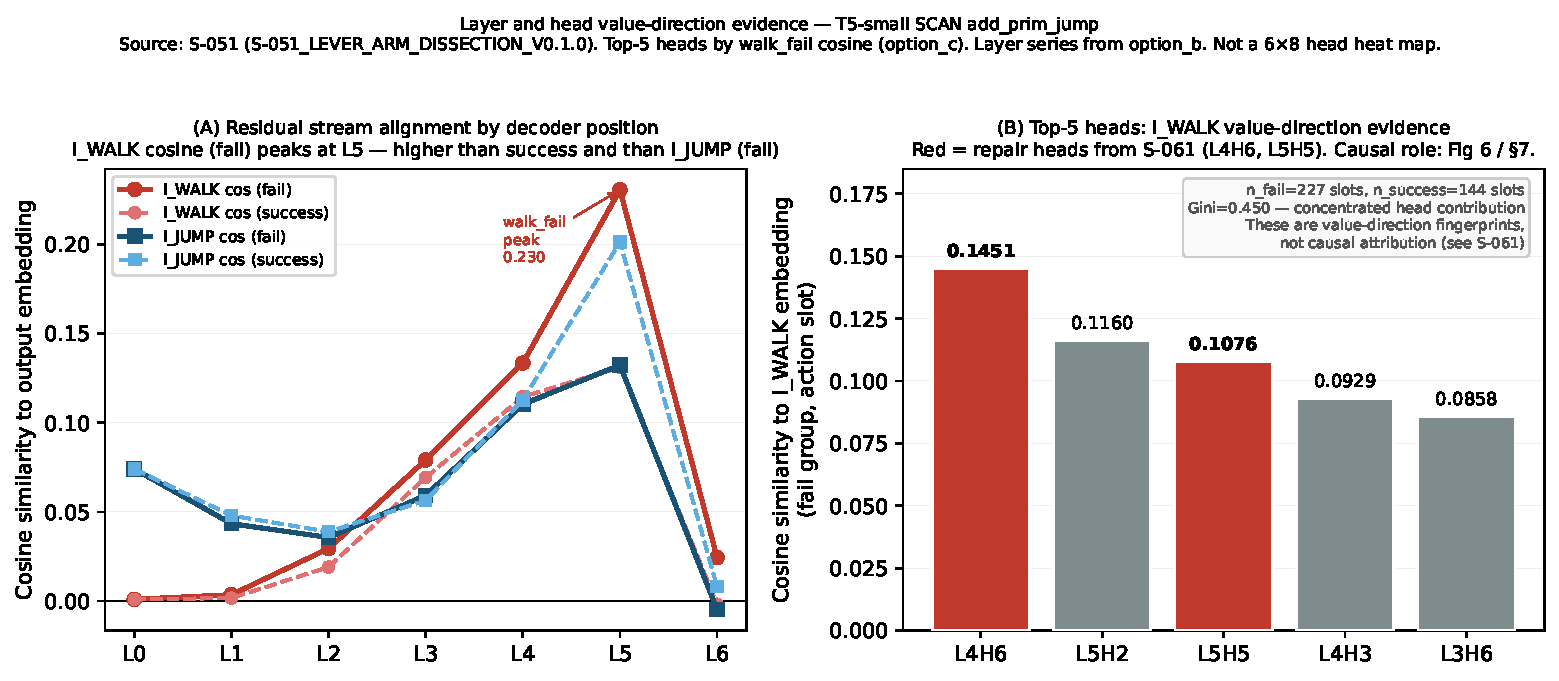
\includegraphics[width=\linewidth]{figures/fig03_value_direction_evidence}
\caption{Layer and head value-direction evidence, T5-small SCAN
\texttt{add\_prim\_jump} (S-051, $n_\text{fail}=227$ action slots,
$n_\text{success}=144$ slots).
Panel~(A): Residual stream cosine similarity to \texttt{I\_WALK} and \texttt{I\_JUMP}
output embeddings by decoder position. In fail cases, \texttt{I\_WALK} alignment peaks
at L5 (0.230), substantially above success-group alignment (0.131) and above
\texttt{I\_JUMP} alignment in fail cases (0.132).
Panel~(B): Top-5 heads by \texttt{I\_WALK} cosine in fail group (option\_c stored
summary; not a complete $6{\times}8$ attribution).
Red bars mark L4H6 and L5H5, identified as primary repair heads in S-061
(\S\ref{sec:repair}~/~Fig.~\ref{fig:dose-response}).
These cosine values are value-direction fingerprints, not causal attribution.
Gini$=0.45$ indicates concentrated head contribution.}
\label{fig:value-direction}
\end{figure}

\subsection{What This Does Not Establish}

The evidence in this section supports a specific chain: the failure is selective and
structural; routing is not the primary discriminator in the stored comparison; and
value-direction evidence points to a small number of heads, especially L4H6 and L5H5,
that attend to the \texttt{jump} encoder token and contribute in the \texttt{I\_WALK}
direction at the action slot.
The following are explicitly \emph{not} established here:

\begin{itemize}
  \item \textbf{Within-category grading of encoder signal.}
    S-043 shows that the encoder categorically marks \texttt{jump} as OOD (between
    groups). S-044 and S-045 found that the encoder does not significantly grade
    failure difficulty \emph{within} the jump-compound category: the OOD signal is
    present but flat across instances.

  \item \textbf{Routing integrity for all failure types.}
    The routing integrity result holds for the stored \texttt{has\_around}=1 fail group
    comparison in S-049 ($n_\text{fail}=50$, $n_\text{success}=25$).
    It does not generalize to other failure types, other group sizes, or other decoder
    layers without further evidence.

  \item \textbf{L4H6 and L5H5 are the only heads involved.}
    Option~C reports the top-5 heads from the stored summary (not a complete
    $6 \times 8$ attribution). L4H3 and L3H6 also appear in the top-5.
    The stored summary does not establish that other heads are uninvolved.

  \item \textbf{Causal attribution from cosine evidence.}
    The cosine alignment of L4H6 and L5H5 toward \texttt{I\_WALK} is directional
    correlation, not causal evidence. The causal claim --- that modifying their
    $W_V$ matrices shifts the action-slot output in the predicted direction ---
    is tested and reported in \S\ref{sec:repair}.
\end{itemize}
